\documentclass[12pt]{article}

\setlength\parindent{0pt}
\newcommand{\myt}[1]{\textbf{\underline{#1}}}

\usepackage{mathtools}
\usepackage{amssymb}
\usepackage{graphicx}

\title{\vspace{-15ex}Math239 Lecture 19\vspace{-1ex}}
\date{June 22md, 2015}
\author{Graham Cooper}

\begin{document}
	\maketitle
	Topics:
	\begin{enumerate}
		\item Cycles
		\item Connectedness
	\end{enumerate}
	
	\section*{Cycles}
	
	\subsection*{Hamilton Cycle}
	
	\myt{Definition:} A hamilton cycle is a cycle that contains every vertex of the graph\\
	
	ie:\\
	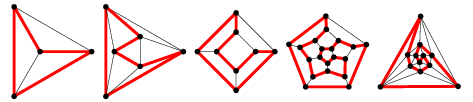
\includegraphics[scale=0.5]{hamilton1.png}\\
	
	Peterson Graph, no hamilton cycle:\\
	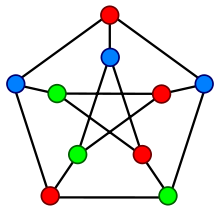
\includegraphics[scale=0.5]{peterson.png}
	
	Traveling salesman problem: Given a list of cities and the distances between each pair of cities, what is the shortest possible route that visits each city exactly once and returns to the origin city?\\
	
	\subsubsection*{Finding a Ham cycle of the shortest length}
	
	Theorem: For $n \geq 2$ the n-cube has a Ham cycle\\
	
	Find a hamilton cycle for the smaller n-cube then link the two new sections together.\\
	
	Proof: By induction on n.\\
	
	For n = 2 it is obviously a ham cycle. as we are just going in a square around the edges. Assume (n-1)-cube has a Ham cycle. The n-cube is built from 2 copies of the (n-1) cube. Take the same Ham-cycle of the (n-1)-cube for both copies. Suppose st is an edge of the Ham cycle for the (n-1)-cube. Then Os, Ot and ls, lt are edges in the n-cube. Remove these two edges and add 0s, ls and ot, lt to get a Ham cycle in the n-cube.\\
	
	\section*{Connectedness}
	
	\myt{Definition:} A graph G is connected if there is a u,v-path for every pair of vertices u,v $\in$ V(G)\\
	
	Theorem: If there exists a vertex u $\in$ V(G) such that a u,v-path exist for all v $\in$ V(G) then G is connected.\\
	
	Proof: \\
	
	Let x,y be any two vertices in G. By assumption, there exists an x,u-path and a u,y-path. By tansitivity, there is an x.y-path so G is connected\
	
	Theorem:: The n-cube is connected\\
	
	Proof: Let $v_0$ be the string of n 0's and let x be any string of length n. Suppose x has k 1's, located at positions $i_1, i_2 ... i_k$. We produce $v_1, v_2, ... v_k$ by letting $v_j$ be the string with exactly j 1's, at positions $i_1, i_2, ... i_j.$ notce that for $j \geq 0$ $v_j$ and $v_{j+1}$ differe in one bit at position $i_{j+1}$ so $v_jv_{j+1}$ is an edge. Hence, $v_0, v_1, v_2...v_k = x$ is a $v_0,x$-path. Therefore the n-cube is connected\\
	
	\section*{Components and Cuts}
	
	\myt{Definition}: A subgraph H of G has vertex set V(H) $\subseteq$ V(G) and E(H) $\subseteq$ E(G) where each edge in E(H) joins two vertices in V(H)\\
	
	Example:\\
	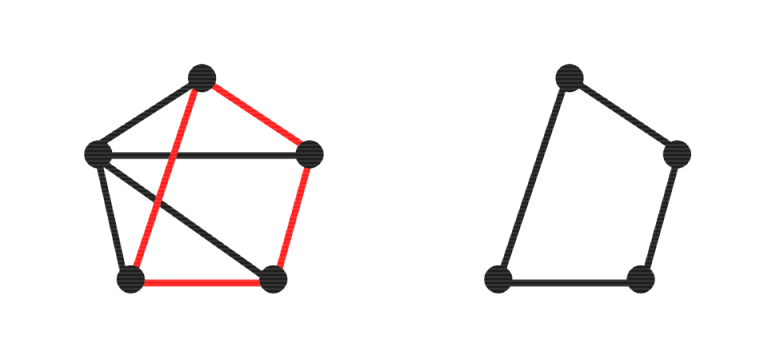
\includegraphics[scale=0.5]{subgraph.png}
	
	
	
	
\end{document}
